% Created by tikzDevice version 0.12.3.1 on 2021-11-28 16:40:07
% !TEX encoding = UTF-8 Unicode
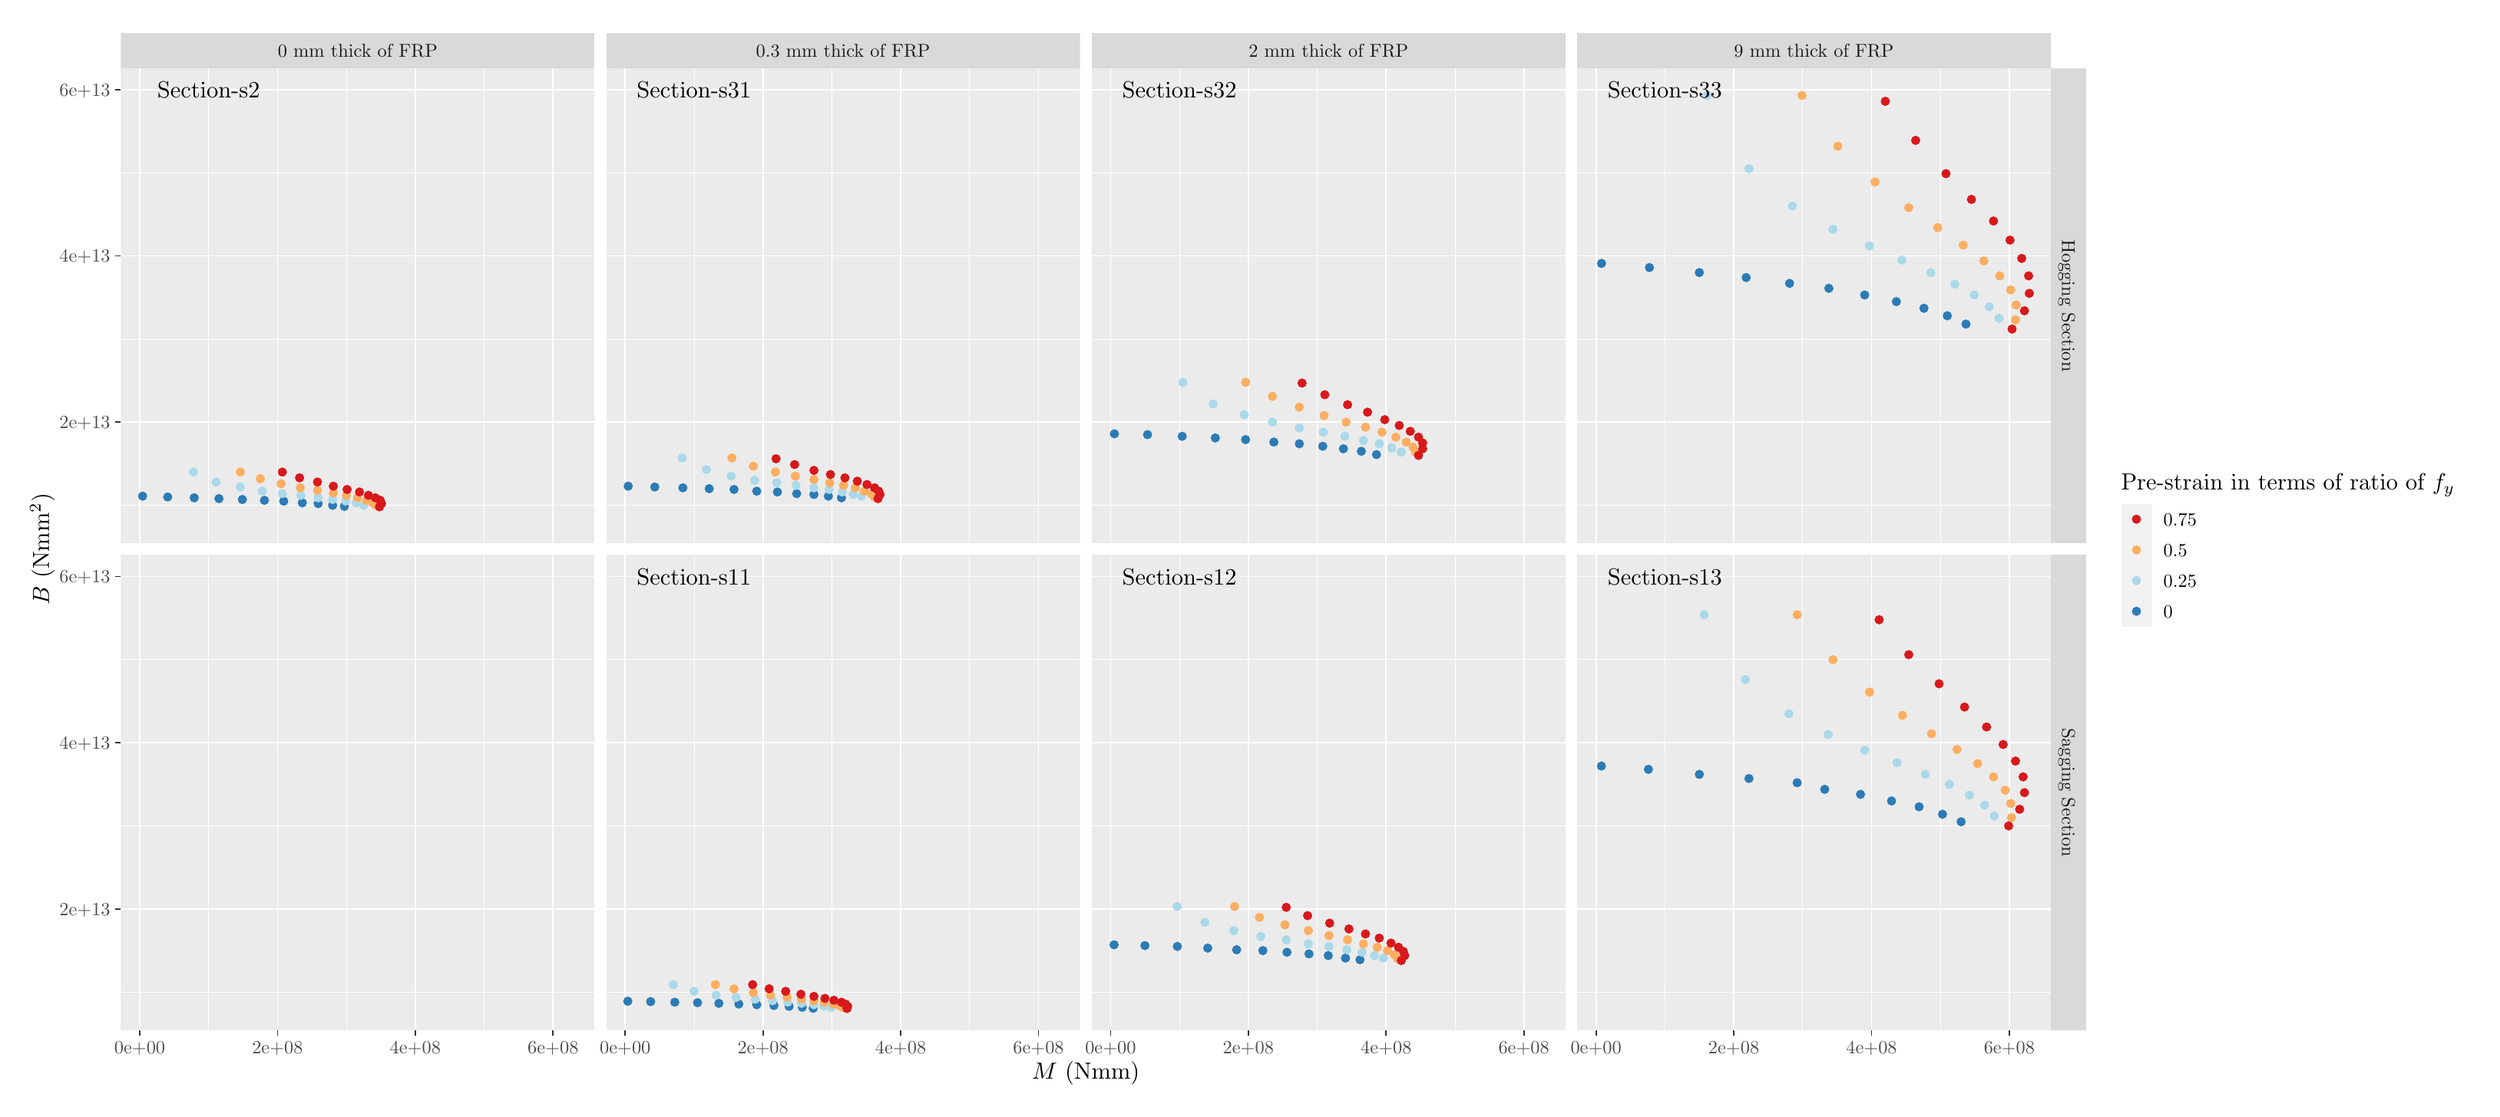
\begin{tikzpicture}[x=1pt,y=1pt]
\definecolor{fillColor}{RGB}{255,255,255}
\path[use as bounding box,fill=fillColor,fill opacity=0.00] (0,0) rectangle (1156.32,505.89);
\begin{scope}
\path[clip] (  0.00,  0.00) rectangle (1156.32,505.89);
\definecolor{drawColor}{RGB}{255,255,255}
\definecolor{fillColor}{RGB}{255,255,255}

\path[draw=drawColor,line width= 0.6pt,line join=round,line cap=round,fill=fillColor] (  0.00,  0.00) rectangle (1156.32,505.89);
\end{scope}
\begin{scope}
\path[clip] ( 46.86,260.00) rectangle (269.81,483.82);
\definecolor{fillColor}{gray}{0.92}

\path[fill=fillColor] ( 46.86,260.00) rectangle (269.81,483.82);
\definecolor{drawColor}{RGB}{255,255,255}

\path[draw=drawColor,line width= 0.3pt,line join=round] ( 46.86,277.89) --
	(269.81,277.89);

\path[draw=drawColor,line width= 0.3pt,line join=round] ( 46.86,356.19) --
	(269.81,356.19);

\path[draw=drawColor,line width= 0.3pt,line join=round] ( 46.86,434.49) --
	(269.81,434.49);

\path[draw=drawColor,line width= 0.3pt,line join=round] ( 88.19,260.00) --
	( 88.19,483.82);

\path[draw=drawColor,line width= 0.3pt,line join=round] (153.03,260.00) --
	(153.03,483.82);

\path[draw=drawColor,line width= 0.3pt,line join=round] (217.86,260.00) --
	(217.86,483.82);

\path[draw=drawColor,line width= 0.6pt,line join=round] ( 46.86,317.04) --
	(269.81,317.04);

\path[draw=drawColor,line width= 0.6pt,line join=round] ( 46.86,395.34) --
	(269.81,395.34);

\path[draw=drawColor,line width= 0.6pt,line join=round] ( 46.86,473.65) --
	(269.81,473.65);

\path[draw=drawColor,line width= 0.6pt,line join=round] ( 55.77,260.00) --
	( 55.77,483.82);

\path[draw=drawColor,line width= 0.6pt,line join=round] (120.61,260.00) --
	(120.61,483.82);

\path[draw=drawColor,line width= 0.6pt,line join=round] (185.44,260.00) --
	(185.44,483.82);

\path[draw=drawColor,line width= 0.6pt,line join=round] (250.28,260.00) --
	(250.28,483.82);
\definecolor{drawColor}{RGB}{44,123,182}
\definecolor{fillColor}{RGB}{44,123,182}

\path[draw=drawColor,line width= 0.4pt,line join=round,line cap=round,fill=fillColor] ( 57.12,282.20) circle (  1.96);

\path[draw=drawColor,line width= 0.4pt,line join=round,line cap=round,fill=fillColor] ( 68.93,281.80) circle (  1.96);

\path[draw=drawColor,line width= 0.4pt,line join=round,line cap=round,fill=fillColor] ( 81.41,281.41) circle (  1.96);

\path[draw=drawColor,line width= 0.4pt,line join=round,line cap=round,fill=fillColor] ( 93.05,281.02) circle (  1.96);

\path[draw=drawColor,line width= 0.4pt,line join=round,line cap=round,fill=fillColor] (104.07,280.63) circle (  1.96);

\path[draw=drawColor,line width= 0.4pt,line join=round,line cap=round,fill=fillColor] (114.45,280.24) circle (  1.96);

\path[draw=drawColor,line width= 0.4pt,line join=round,line cap=round,fill=fillColor] (123.53,279.85) circle (  1.96);

\path[draw=drawColor,line width= 0.4pt,line join=round,line cap=round,fill=fillColor] (132.28,279.06) circle (  1.96);

\path[draw=drawColor,line width= 0.4pt,line join=round,line cap=round,fill=fillColor] (139.73,278.67) circle (  1.96);

\path[draw=drawColor,line width= 0.4pt,line join=round,line cap=round,fill=fillColor] (146.54,277.89) circle (  1.96);

\path[draw=drawColor,line width= 0.4pt,line join=round,line cap=round,fill=fillColor] (152.05,277.38) circle (  1.96);
\definecolor{drawColor}{RGB}{171,217,233}
\definecolor{fillColor}{RGB}{171,217,233}

\path[draw=drawColor,line width= 0.4pt,line join=round,line cap=round,fill=fillColor] ( 81.09,293.55) circle (  1.96);

\path[draw=drawColor,line width= 0.4pt,line join=round,line cap=round,fill=fillColor] ( 91.76,288.85) circle (  1.96);

\path[draw=drawColor,line width= 0.4pt,line join=round,line cap=round,fill=fillColor] (103.10,286.50) circle (  1.96);

\path[draw=drawColor,line width= 0.4pt,line join=round,line cap=round,fill=fillColor] (113.48,284.54) circle (  1.96);

\path[draw=drawColor,line width= 0.4pt,line join=round,line cap=round,fill=fillColor] (122.88,283.37) circle (  1.96);

\path[draw=drawColor,line width= 0.4pt,line join=round,line cap=round,fill=fillColor] (131.63,282.59) circle (  1.96);

\path[draw=drawColor,line width= 0.4pt,line join=round,line cap=round,fill=fillColor] (139.73,281.41) circle (  1.96);

\path[draw=drawColor,line width= 0.4pt,line join=round,line cap=round,fill=fillColor] (146.54,280.63) circle (  1.96);

\path[draw=drawColor,line width= 0.4pt,line join=round,line cap=round,fill=fillColor] (152.70,279.85) circle (  1.96);

\path[draw=drawColor,line width= 0.4pt,line join=round,line cap=round,fill=fillColor] (157.56,279.06) circle (  1.96);

\path[draw=drawColor,line width= 0.4pt,line join=round,line cap=round,fill=fillColor] (161.13,277.89) circle (  1.96);
\definecolor{drawColor}{RGB}{253,174,97}
\definecolor{fillColor}{RGB}{253,174,97}

\path[draw=drawColor,line width= 0.4pt,line join=round,line cap=round,fill=fillColor] (103.10,293.55) circle (  1.96);

\path[draw=drawColor,line width= 0.4pt,line join=round,line cap=round,fill=fillColor] (112.50,290.42) circle (  1.96);

\path[draw=drawColor,line width= 0.4pt,line join=round,line cap=round,fill=fillColor] (122.23,288.07) circle (  1.96);

\path[draw=drawColor,line width= 0.4pt,line join=round,line cap=round,fill=fillColor] (131.31,286.11) circle (  1.96);

\path[draw=drawColor,line width= 0.4pt,line join=round,line cap=round,fill=fillColor] (139.41,284.94) circle (  1.96);

\path[draw=drawColor,line width= 0.4pt,line join=round,line cap=round,fill=fillColor] (146.87,283.76) circle (  1.96);

\path[draw=drawColor,line width= 0.4pt,line join=round,line cap=round,fill=fillColor] (153.03,282.59) circle (  1.96);

\path[draw=drawColor,line width= 0.4pt,line join=round,line cap=round,fill=fillColor] (158.21,281.41) circle (  1.96);

\path[draw=drawColor,line width= 0.4pt,line join=round,line cap=round,fill=fillColor] (162.43,280.24) circle (  1.96);

\path[draw=drawColor,line width= 0.4pt,line join=round,line cap=round,fill=fillColor] (165.34,279.06) circle (  1.96);

\path[draw=drawColor,line width= 0.4pt,line join=round,line cap=round,fill=fillColor] (166.96,277.85) circle (  1.96);
\definecolor{drawColor}{RGB}{215,25,28}
\definecolor{fillColor}{RGB}{215,25,28}

\path[draw=drawColor,line width= 0.4pt,line join=round,line cap=round,fill=fillColor] (122.88,293.55) circle (  1.96);

\path[draw=drawColor,line width= 0.4pt,line join=round,line cap=round,fill=fillColor] (130.98,290.81) circle (  1.96);

\path[draw=drawColor,line width= 0.4pt,line join=round,line cap=round,fill=fillColor] (139.41,288.85) circle (  1.96);

\path[draw=drawColor,line width= 0.4pt,line join=round,line cap=round,fill=fillColor] (146.87,286.89) circle (  1.96);

\path[draw=drawColor,line width= 0.4pt,line join=round,line cap=round,fill=fillColor] (153.35,285.33) circle (  1.96);

\path[draw=drawColor,line width= 0.4pt,line join=round,line cap=round,fill=fillColor] (159.18,284.15) circle (  1.96);

\path[draw=drawColor,line width= 0.4pt,line join=round,line cap=round,fill=fillColor] (163.40,282.59) circle (  1.96);

\path[draw=drawColor,line width= 0.4pt,line join=round,line cap=round,fill=fillColor] (166.64,281.41) circle (  1.96);

\path[draw=drawColor,line width= 0.4pt,line join=round,line cap=round,fill=fillColor] (168.91,280.24) circle (  1.96);

\path[draw=drawColor,line width= 0.4pt,line join=round,line cap=round,fill=fillColor] (169.56,278.67) circle (  1.96);

\path[draw=drawColor,line width= 0.4pt,line join=round,line cap=round,fill=fillColor] (168.59,277.14) circle (  1.96);
\definecolor{drawColor}{RGB}{0,0,0}

\node[text=drawColor,anchor=base,inner sep=0pt, outer sep=0pt, scale=  1.10] at ( 88.19,469.84) {Section-s2};
\end{scope}
\begin{scope}
\path[clip] ( 46.86, 30.69) rectangle (269.81,254.50);
\definecolor{fillColor}{gray}{0.92}

\path[fill=fillColor] ( 46.86, 30.69) rectangle (269.81,254.50);
\definecolor{drawColor}{RGB}{255,255,255}

\path[draw=drawColor,line width= 0.3pt,line join=round] ( 46.86, 48.57) --
	(269.81, 48.57);

\path[draw=drawColor,line width= 0.3pt,line join=round] ( 46.86,126.87) --
	(269.81,126.87);

\path[draw=drawColor,line width= 0.3pt,line join=round] ( 46.86,205.18) --
	(269.81,205.18);

\path[draw=drawColor,line width= 0.3pt,line join=round] ( 88.19, 30.69) --
	( 88.19,254.50);

\path[draw=drawColor,line width= 0.3pt,line join=round] (153.03, 30.69) --
	(153.03,254.50);

\path[draw=drawColor,line width= 0.3pt,line join=round] (217.86, 30.69) --
	(217.86,254.50);

\path[draw=drawColor,line width= 0.6pt,line join=round] ( 46.86, 87.72) --
	(269.81, 87.72);

\path[draw=drawColor,line width= 0.6pt,line join=round] ( 46.86,166.03) --
	(269.81,166.03);

\path[draw=drawColor,line width= 0.6pt,line join=round] ( 46.86,244.33) --
	(269.81,244.33);

\path[draw=drawColor,line width= 0.6pt,line join=round] ( 55.77, 30.69) --
	( 55.77,254.50);

\path[draw=drawColor,line width= 0.6pt,line join=round] (120.61, 30.69) --
	(120.61,254.50);

\path[draw=drawColor,line width= 0.6pt,line join=round] (185.44, 30.69) --
	(185.44,254.50);

\path[draw=drawColor,line width= 0.6pt,line join=round] (250.28, 30.69) --
	(250.28,254.50);
\end{scope}
\begin{scope}
\path[clip] (275.31,260.00) rectangle (498.26,483.82);
\definecolor{fillColor}{gray}{0.92}

\path[fill=fillColor] (275.31,260.00) rectangle (498.26,483.82);
\definecolor{drawColor}{RGB}{255,255,255}

\path[draw=drawColor,line width= 0.3pt,line join=round] (275.31,277.89) --
	(498.26,277.89);

\path[draw=drawColor,line width= 0.3pt,line join=round] (275.31,356.19) --
	(498.26,356.19);

\path[draw=drawColor,line width= 0.3pt,line join=round] (275.31,434.49) --
	(498.26,434.49);

\path[draw=drawColor,line width= 0.3pt,line join=round] (316.64,260.00) --
	(316.64,483.82);

\path[draw=drawColor,line width= 0.3pt,line join=round] (381.47,260.00) --
	(381.47,483.82);

\path[draw=drawColor,line width= 0.3pt,line join=round] (446.31,260.00) --
	(446.31,483.82);

\path[draw=drawColor,line width= 0.6pt,line join=round] (275.31,317.04) --
	(498.26,317.04);

\path[draw=drawColor,line width= 0.6pt,line join=round] (275.31,395.34) --
	(498.26,395.34);

\path[draw=drawColor,line width= 0.6pt,line join=round] (275.31,473.65) --
	(498.26,473.65);

\path[draw=drawColor,line width= 0.6pt,line join=round] (284.22,260.00) --
	(284.22,483.82);

\path[draw=drawColor,line width= 0.6pt,line join=round] (349.06,260.00) --
	(349.06,483.82);

\path[draw=drawColor,line width= 0.6pt,line join=round] (413.89,260.00) --
	(413.89,483.82);

\path[draw=drawColor,line width= 0.6pt,line join=round] (478.73,260.00) --
	(478.73,483.82);
\definecolor{drawColor}{RGB}{44,123,182}
\definecolor{fillColor}{RGB}{44,123,182}

\path[draw=drawColor,line width= 0.4pt,line join=round,line cap=round,fill=fillColor] (285.65,286.89) circle (  1.96);

\path[draw=drawColor,line width= 0.4pt,line join=round,line cap=round,fill=fillColor] (298.16,286.50) circle (  1.96);

\path[draw=drawColor,line width= 0.4pt,line join=round,line cap=round,fill=fillColor] (311.35,286.11) circle (  1.96);

\path[draw=drawColor,line width= 0.4pt,line join=round,line cap=round,fill=fillColor] (323.77,285.72) circle (  1.96);

\path[draw=drawColor,line width= 0.4pt,line join=round,line cap=round,fill=fillColor] (335.44,285.33) circle (  1.96);

\path[draw=drawColor,line width= 0.4pt,line join=round,line cap=round,fill=fillColor] (346.14,284.54) circle (  1.96);

\path[draw=drawColor,line width= 0.4pt,line join=round,line cap=round,fill=fillColor] (355.86,284.15) circle (  1.96);

\path[draw=drawColor,line width= 0.4pt,line join=round,line cap=round,fill=fillColor] (364.94,283.37) circle (  1.96);

\path[draw=drawColor,line width= 0.4pt,line join=round,line cap=round,fill=fillColor] (373.05,282.98) circle (  1.96);

\path[draw=drawColor,line width= 0.4pt,line join=round,line cap=round,fill=fillColor] (379.85,282.20) circle (  1.96);

\path[draw=drawColor,line width= 0.4pt,line join=round,line cap=round,fill=fillColor] (386.01,281.41) circle (  1.96);
\definecolor{drawColor}{RGB}{171,217,233}
\definecolor{fillColor}{RGB}{171,217,233}

\path[draw=drawColor,line width= 0.4pt,line join=round,line cap=round,fill=fillColor] (311.10,300.20) circle (  1.96);

\path[draw=drawColor,line width= 0.4pt,line join=round,line cap=round,fill=fillColor] (322.47,294.72) circle (  1.96);

\path[draw=drawColor,line width= 0.4pt,line join=round,line cap=round,fill=fillColor] (334.14,291.59) circle (  1.96);

\path[draw=drawColor,line width= 0.4pt,line join=round,line cap=round,fill=fillColor] (345.17,289.63) circle (  1.96);

\path[draw=drawColor,line width= 0.4pt,line join=round,line cap=round,fill=fillColor] (355.54,288.46) circle (  1.96);

\path[draw=drawColor,line width= 0.4pt,line join=round,line cap=round,fill=fillColor] (364.62,287.28) circle (  1.96);

\path[draw=drawColor,line width= 0.4pt,line join=round,line cap=round,fill=fillColor] (373.05,286.11) circle (  1.96);

\path[draw=drawColor,line width= 0.4pt,line join=round,line cap=round,fill=fillColor] (380.18,285.33) circle (  1.96);

\path[draw=drawColor,line width= 0.4pt,line join=round,line cap=round,fill=fillColor] (386.34,284.15) circle (  1.96);

\path[draw=drawColor,line width= 0.4pt,line join=round,line cap=round,fill=fillColor] (391.52,282.98) circle (  1.96);

\path[draw=drawColor,line width= 0.4pt,line join=round,line cap=round,fill=fillColor] (395.41,282.20) circle (  1.96);
\definecolor{drawColor}{RGB}{253,174,97}
\definecolor{fillColor}{RGB}{253,174,97}

\path[draw=drawColor,line width= 0.4pt,line join=round,line cap=round,fill=fillColor] (334.47,300.20) circle (  1.96);

\path[draw=drawColor,line width= 0.4pt,line join=round,line cap=round,fill=fillColor] (344.52,296.29) circle (  1.96);

\path[draw=drawColor,line width= 0.4pt,line join=round,line cap=round,fill=fillColor] (354.89,293.55) circle (  1.96);

\path[draw=drawColor,line width= 0.4pt,line join=round,line cap=round,fill=fillColor] (364.29,291.59) circle (  1.96);

\path[draw=drawColor,line width= 0.4pt,line join=round,line cap=round,fill=fillColor] (373.05,290.03) circle (  1.96);

\path[draw=drawColor,line width= 0.4pt,line join=round,line cap=round,fill=fillColor] (380.50,288.46) circle (  1.96);

\path[draw=drawColor,line width= 0.4pt,line join=round,line cap=round,fill=fillColor] (386.98,287.28) circle (  1.96);

\path[draw=drawColor,line width= 0.4pt,line join=round,line cap=round,fill=fillColor] (392.50,286.11) circle (  1.96);

\path[draw=drawColor,line width= 0.4pt,line join=round,line cap=round,fill=fillColor] (396.71,284.54) circle (  1.96);

\path[draw=drawColor,line width= 0.4pt,line join=round,line cap=round,fill=fillColor] (399.95,283.37) circle (  1.96);

\path[draw=drawColor,line width= 0.4pt,line join=round,line cap=round,fill=fillColor] (401.57,281.80) circle (  1.96);
\definecolor{drawColor}{RGB}{215,25,28}
\definecolor{fillColor}{RGB}{215,25,28}

\path[draw=drawColor,line width= 0.4pt,line join=round,line cap=round,fill=fillColor] (355.22,299.81) circle (  1.96);

\path[draw=drawColor,line width= 0.4pt,line join=round,line cap=round,fill=fillColor] (363.97,297.07) circle (  1.96);

\path[draw=drawColor,line width= 0.4pt,line join=round,line cap=round,fill=fillColor] (373.05,294.33) circle (  1.96);

\path[draw=drawColor,line width= 0.4pt,line join=round,line cap=round,fill=fillColor] (380.83,292.37) circle (  1.96);

\path[draw=drawColor,line width= 0.4pt,line join=round,line cap=round,fill=fillColor] (387.63,290.81) circle (  1.96);

\path[draw=drawColor,line width= 0.4pt,line join=round,line cap=round,fill=fillColor] (393.47,289.24) circle (  1.96);

\path[draw=drawColor,line width= 0.4pt,line join=round,line cap=round,fill=fillColor] (398.01,287.68) circle (  1.96);

\path[draw=drawColor,line width= 0.4pt,line join=round,line cap=round,fill=fillColor] (401.57,286.11) circle (  1.96);

\path[draw=drawColor,line width= 0.4pt,line join=round,line cap=round,fill=fillColor] (403.52,284.54) circle (  1.96);

\path[draw=drawColor,line width= 0.4pt,line join=round,line cap=round,fill=fillColor] (404.17,282.98) circle (  1.96);

\path[draw=drawColor,line width= 0.4pt,line join=round,line cap=round,fill=fillColor] (403.19,281.02) circle (  1.96);
\definecolor{drawColor}{RGB}{0,0,0}

\node[text=drawColor,anchor=base,inner sep=0pt, outer sep=0pt, scale=  1.10] at (316.64,469.84) {Section-s31};
\end{scope}
\begin{scope}
\path[clip] (275.31, 30.69) rectangle (498.26,254.50);
\definecolor{fillColor}{gray}{0.92}

\path[fill=fillColor] (275.31, 30.69) rectangle (498.26,254.50);
\definecolor{drawColor}{RGB}{255,255,255}

\path[draw=drawColor,line width= 0.3pt,line join=round] (275.31, 48.57) --
	(498.26, 48.57);

\path[draw=drawColor,line width= 0.3pt,line join=round] (275.31,126.87) --
	(498.26,126.87);

\path[draw=drawColor,line width= 0.3pt,line join=round] (275.31,205.18) --
	(498.26,205.18);

\path[draw=drawColor,line width= 0.3pt,line join=round] (316.64, 30.69) --
	(316.64,254.50);

\path[draw=drawColor,line width= 0.3pt,line join=round] (381.47, 30.69) --
	(381.47,254.50);

\path[draw=drawColor,line width= 0.3pt,line join=round] (446.31, 30.69) --
	(446.31,254.50);

\path[draw=drawColor,line width= 0.6pt,line join=round] (275.31, 87.72) --
	(498.26, 87.72);

\path[draw=drawColor,line width= 0.6pt,line join=round] (275.31,166.03) --
	(498.26,166.03);

\path[draw=drawColor,line width= 0.6pt,line join=round] (275.31,244.33) --
	(498.26,244.33);

\path[draw=drawColor,line width= 0.6pt,line join=round] (284.22, 30.69) --
	(284.22,254.50);

\path[draw=drawColor,line width= 0.6pt,line join=round] (349.06, 30.69) --
	(349.06,254.50);

\path[draw=drawColor,line width= 0.6pt,line join=round] (413.89, 30.69) --
	(413.89,254.50);

\path[draw=drawColor,line width= 0.6pt,line join=round] (478.73, 30.69) --
	(478.73,254.50);
\definecolor{drawColor}{RGB}{44,123,182}
\definecolor{fillColor}{RGB}{44,123,182}

\path[draw=drawColor,line width= 0.4pt,line join=round,line cap=round,fill=fillColor] (285.45, 44.30) circle (  1.96);

\path[draw=drawColor,line width= 0.4pt,line join=round,line cap=round,fill=fillColor] (296.22, 44.11) circle (  1.96);

\path[draw=drawColor,line width= 0.4pt,line join=round,line cap=round,fill=fillColor] (307.56, 43.83) circle (  1.96);

\path[draw=drawColor,line width= 0.4pt,line join=round,line cap=round,fill=fillColor] (318.26, 43.60) circle (  1.96);

\path[draw=drawColor,line width= 0.4pt,line join=round,line cap=round,fill=fillColor] (328.31, 43.29) circle (  1.96);

\path[draw=drawColor,line width= 0.4pt,line join=round,line cap=round,fill=fillColor] (337.71, 42.97) circle (  1.96);

\path[draw=drawColor,line width= 0.4pt,line join=round,line cap=round,fill=fillColor] (346.14, 42.66) circle (  1.96);

\path[draw=drawColor,line width= 0.4pt,line join=round,line cap=round,fill=fillColor] (354.24, 42.27) circle (  1.96);

\path[draw=drawColor,line width= 0.4pt,line join=round,line cap=round,fill=fillColor] (361.37, 41.88) circle (  1.96);

\path[draw=drawColor,line width= 0.4pt,line join=round,line cap=round,fill=fillColor] (367.53, 41.45) circle (  1.96);

\path[draw=drawColor,line width= 0.4pt,line join=round,line cap=round,fill=fillColor] (372.72, 40.98) circle (  1.96);
\definecolor{drawColor}{RGB}{171,217,233}
\definecolor{fillColor}{RGB}{171,217,233}

\path[draw=drawColor,line width= 0.4pt,line join=round,line cap=round,fill=fillColor] (306.88, 52.10) circle (  1.96);

\path[draw=drawColor,line width= 0.4pt,line join=round,line cap=round,fill=fillColor] (316.64, 48.96) circle (  1.96);

\path[draw=drawColor,line width= 0.4pt,line join=round,line cap=round,fill=fillColor] (327.01, 47.16) circle (  1.96);

\path[draw=drawColor,line width= 0.4pt,line join=round,line cap=round,fill=fillColor] (336.41, 46.07) circle (  1.96);

\path[draw=drawColor,line width= 0.4pt,line join=round,line cap=round,fill=fillColor] (345.49, 45.24) circle (  1.96);

\path[draw=drawColor,line width= 0.4pt,line join=round,line cap=round,fill=fillColor] (353.59, 44.54) circle (  1.96);

\path[draw=drawColor,line width= 0.4pt,line join=round,line cap=round,fill=fillColor] (360.73, 43.87) circle (  1.96);

\path[draw=drawColor,line width= 0.4pt,line join=round,line cap=round,fill=fillColor] (367.21, 43.29) circle (  1.96);

\path[draw=drawColor,line width= 0.4pt,line join=round,line cap=round,fill=fillColor] (373.05, 42.66) circle (  1.96);

\path[draw=drawColor,line width= 0.4pt,line join=round,line cap=round,fill=fillColor] (377.58, 42.03) circle (  1.96);

\path[draw=drawColor,line width= 0.4pt,line join=round,line cap=round,fill=fillColor] (381.15, 41.37) circle (  1.96);
\definecolor{drawColor}{RGB}{253,174,97}
\definecolor{fillColor}{RGB}{253,174,97}

\path[draw=drawColor,line width= 0.4pt,line join=round,line cap=round,fill=fillColor] (326.69, 52.10) circle (  1.96);

\path[draw=drawColor,line width= 0.4pt,line join=round,line cap=round,fill=fillColor] (335.44, 50.14) circle (  1.96);

\path[draw=drawColor,line width= 0.4pt,line join=round,line cap=round,fill=fillColor] (344.52, 48.34) circle (  1.96);

\path[draw=drawColor,line width= 0.4pt,line join=round,line cap=round,fill=fillColor] (352.62, 47.16) circle (  1.96);

\path[draw=drawColor,line width= 0.4pt,line join=round,line cap=round,fill=fillColor] (360.40, 46.18) circle (  1.96);

\path[draw=drawColor,line width= 0.4pt,line join=round,line cap=round,fill=fillColor] (367.21, 45.32) circle (  1.96);

\path[draw=drawColor,line width= 0.4pt,line join=round,line cap=round,fill=fillColor] (373.05, 44.50) circle (  1.96);

\path[draw=drawColor,line width= 0.4pt,line join=round,line cap=round,fill=fillColor] (377.91, 43.76) circle (  1.96);

\path[draw=drawColor,line width= 0.4pt,line join=round,line cap=round,fill=fillColor] (382.12, 42.97) circle (  1.96);

\path[draw=drawColor,line width= 0.4pt,line join=round,line cap=round,fill=fillColor] (385.04, 42.19) circle (  1.96);

\path[draw=drawColor,line width= 0.4pt,line join=round,line cap=round,fill=fillColor] (386.66, 41.33) circle (  1.96);
\definecolor{drawColor}{RGB}{215,25,28}
\definecolor{fillColor}{RGB}{215,25,28}

\path[draw=drawColor,line width= 0.4pt,line join=round,line cap=round,fill=fillColor] (344.19, 52.10) circle (  1.96);

\path[draw=drawColor,line width= 0.4pt,line join=round,line cap=round,fill=fillColor] (351.97, 50.14) circle (  1.96);

\path[draw=drawColor,line width= 0.4pt,line join=round,line cap=round,fill=fillColor] (359.75, 48.96) circle (  1.96);

\path[draw=drawColor,line width= 0.4pt,line join=round,line cap=round,fill=fillColor] (366.89, 47.59) circle (  1.96);

\path[draw=drawColor,line width= 0.4pt,line join=round,line cap=round,fill=fillColor] (373.05, 46.58) circle (  1.96);

\path[draw=drawColor,line width= 0.4pt,line join=round,line cap=round,fill=fillColor] (378.23, 45.64) circle (  1.96);

\path[draw=drawColor,line width= 0.4pt,line join=round,line cap=round,fill=fillColor] (382.45, 44.74) circle (  1.96);

\path[draw=drawColor,line width= 0.4pt,line join=round,line cap=round,fill=fillColor] (386.01, 43.83) circle (  1.96);

\path[draw=drawColor,line width= 0.4pt,line join=round,line cap=round,fill=fillColor] (387.96, 42.90) circle (  1.96);

\path[draw=drawColor,line width= 0.4pt,line join=round,line cap=round,fill=fillColor] (388.93, 41.92) circle (  1.96);

\path[draw=drawColor,line width= 0.4pt,line join=round,line cap=round,fill=fillColor] (388.61, 40.86) circle (  1.96);
\definecolor{drawColor}{RGB}{0,0,0}

\node[text=drawColor,anchor=base,inner sep=0pt, outer sep=0pt, scale=  1.10] at (316.64,240.53) {Section-s11};
\end{scope}
\begin{scope}
\path[clip] (503.76,260.00) rectangle (726.71,483.82);
\definecolor{fillColor}{gray}{0.92}

\path[fill=fillColor] (503.76,260.00) rectangle (726.71,483.82);
\definecolor{drawColor}{RGB}{255,255,255}

\path[draw=drawColor,line width= 0.3pt,line join=round] (503.76,277.89) --
	(726.71,277.89);

\path[draw=drawColor,line width= 0.3pt,line join=round] (503.76,356.19) --
	(726.71,356.19);

\path[draw=drawColor,line width= 0.3pt,line join=round] (503.76,434.49) --
	(726.71,434.49);

\path[draw=drawColor,line width= 0.3pt,line join=round] (545.09,260.00) --
	(545.09,483.82);

\path[draw=drawColor,line width= 0.3pt,line join=round] (609.92,260.00) --
	(609.92,483.82);

\path[draw=drawColor,line width= 0.3pt,line join=round] (674.76,260.00) --
	(674.76,483.82);

\path[draw=drawColor,line width= 0.6pt,line join=round] (503.76,317.04) --
	(726.71,317.04);

\path[draw=drawColor,line width= 0.6pt,line join=round] (503.76,395.34) --
	(726.71,395.34);

\path[draw=drawColor,line width= 0.6pt,line join=round] (503.76,473.65) --
	(726.71,473.65);

\path[draw=drawColor,line width= 0.6pt,line join=round] (512.67,260.00) --
	(512.67,483.82);

\path[draw=drawColor,line width= 0.6pt,line join=round] (577.50,260.00) --
	(577.50,483.82);

\path[draw=drawColor,line width= 0.6pt,line join=round] (642.34,260.00) --
	(642.34,483.82);

\path[draw=drawColor,line width= 0.6pt,line join=round] (707.17,260.00) --
	(707.17,483.82);
\definecolor{drawColor}{RGB}{44,123,182}
\definecolor{fillColor}{RGB}{44,123,182}

\path[draw=drawColor,line width= 0.4pt,line join=round,line cap=round,fill=fillColor] (514.45,311.56) circle (  1.96);

\path[draw=drawColor,line width= 0.4pt,line join=round,line cap=round,fill=fillColor] (530.05,311.17) circle (  1.96);

\path[draw=drawColor,line width= 0.4pt,line join=round,line cap=round,fill=fillColor] (546.38,310.38) circle (  1.96);

\path[draw=drawColor,line width= 0.4pt,line join=round,line cap=round,fill=fillColor] (561.94,309.60) circle (  1.96);

\path[draw=drawColor,line width= 0.4pt,line join=round,line cap=round,fill=fillColor] (576.21,308.82) circle (  1.96);

\path[draw=drawColor,line width= 0.4pt,line join=round,line cap=round,fill=fillColor] (589.50,307.64) circle (  1.96);

\path[draw=drawColor,line width= 0.4pt,line join=round,line cap=round,fill=fillColor] (601.49,306.86) circle (  1.96);

\path[draw=drawColor,line width= 0.4pt,line join=round,line cap=round,fill=fillColor] (612.52,305.69) circle (  1.96);

\path[draw=drawColor,line width= 0.4pt,line join=round,line cap=round,fill=fillColor] (622.24,304.51) circle (  1.96);

\path[draw=drawColor,line width= 0.4pt,line join=round,line cap=round,fill=fillColor] (630.67,303.34) circle (  1.96);

\path[draw=drawColor,line width= 0.4pt,line join=round,line cap=round,fill=fillColor] (637.80,301.77) circle (  1.96);
\definecolor{drawColor}{RGB}{171,217,233}
\definecolor{fillColor}{RGB}{171,217,233}

\path[draw=drawColor,line width= 0.4pt,line join=round,line cap=round,fill=fillColor] (546.71,335.83) circle (  1.96);

\path[draw=drawColor,line width= 0.4pt,line join=round,line cap=round,fill=fillColor] (560.97,325.65) circle (  1.96);

\path[draw=drawColor,line width= 0.4pt,line join=round,line cap=round,fill=fillColor] (575.56,320.56) circle (  1.96);

\path[draw=drawColor,line width= 0.4pt,line join=round,line cap=round,fill=fillColor] (588.85,317.04) circle (  1.96);

\path[draw=drawColor,line width= 0.4pt,line join=round,line cap=round,fill=fillColor] (601.49,314.30) circle (  1.96);

\path[draw=drawColor,line width= 0.4pt,line join=round,line cap=round,fill=fillColor] (612.84,312.34) circle (  1.96);

\path[draw=drawColor,line width= 0.4pt,line join=round,line cap=round,fill=fillColor] (622.89,310.38) circle (  1.96);

\path[draw=drawColor,line width= 0.4pt,line join=round,line cap=round,fill=fillColor] (631.64,308.43) circle (  1.96);

\path[draw=drawColor,line width= 0.4pt,line join=round,line cap=round,fill=fillColor] (639.10,306.86) circle (  1.96);

\path[draw=drawColor,line width= 0.4pt,line join=round,line cap=round,fill=fillColor] (644.93,304.90) circle (  1.96);

\path[draw=drawColor,line width= 0.4pt,line join=round,line cap=round,fill=fillColor] (649.47,302.95) circle (  1.96);
\definecolor{drawColor}{RGB}{253,174,97}
\definecolor{fillColor}{RGB}{253,174,97}

\path[draw=drawColor,line width= 0.4pt,line join=round,line cap=round,fill=fillColor] (576.21,335.83) circle (  1.96);

\path[draw=drawColor,line width= 0.4pt,line join=round,line cap=round,fill=fillColor] (588.85,329.18) circle (  1.96);

\path[draw=drawColor,line width= 0.4pt,line join=round,line cap=round,fill=fillColor] (601.49,324.09) circle (  1.96);

\path[draw=drawColor,line width= 0.4pt,line join=round,line cap=round,fill=fillColor] (613.16,320.17) circle (  1.96);

\path[draw=drawColor,line width= 0.4pt,line join=round,line cap=round,fill=fillColor] (623.54,317.04) circle (  1.96);

\path[draw=drawColor,line width= 0.4pt,line join=round,line cap=round,fill=fillColor] (632.61,314.69) circle (  1.96);

\path[draw=drawColor,line width= 0.4pt,line join=round,line cap=round,fill=fillColor] (640.39,312.34) circle (  1.96);

\path[draw=drawColor,line width= 0.4pt,line join=round,line cap=round,fill=fillColor] (646.88,309.99) circle (  1.96);

\path[draw=drawColor,line width= 0.4pt,line join=round,line cap=round,fill=fillColor] (651.74,307.64) circle (  1.96);

\path[draw=drawColor,line width= 0.4pt,line join=round,line cap=round,fill=fillColor] (654.98,305.29) circle (  1.96);

\path[draw=drawColor,line width= 0.4pt,line join=round,line cap=round,fill=fillColor] (656.28,302.95) circle (  1.96);
\definecolor{drawColor}{RGB}{215,25,28}
\definecolor{fillColor}{RGB}{215,25,28}

\path[draw=drawColor,line width= 0.4pt,line join=round,line cap=round,fill=fillColor] (602.79,335.44) circle (  1.96);

\path[draw=drawColor,line width= 0.4pt,line join=round,line cap=round,fill=fillColor] (613.49,329.96) circle (  1.96);

\path[draw=drawColor,line width= 0.4pt,line join=round,line cap=round,fill=fillColor] (624.19,325.26) circle (  1.96);

\path[draw=drawColor,line width= 0.4pt,line join=round,line cap=round,fill=fillColor] (633.59,321.74) circle (  1.96);

\path[draw=drawColor,line width= 0.4pt,line join=round,line cap=round,fill=fillColor] (641.69,318.21) circle (  1.96);

\path[draw=drawColor,line width= 0.4pt,line join=round,line cap=round,fill=fillColor] (648.50,315.47) circle (  1.96);

\path[draw=drawColor,line width= 0.4pt,line join=round,line cap=round,fill=fillColor] (653.69,312.73) circle (  1.96);

\path[draw=drawColor,line width= 0.4pt,line join=round,line cap=round,fill=fillColor] (657.58,309.99) circle (  1.96);

\path[draw=drawColor,line width= 0.4pt,line join=round,line cap=round,fill=fillColor] (659.52,307.25) circle (  1.96);

\path[draw=drawColor,line width= 0.4pt,line join=round,line cap=round,fill=fillColor] (659.52,304.51) circle (  1.96);

\path[draw=drawColor,line width= 0.4pt,line join=round,line cap=round,fill=fillColor] (657.58,301.38) circle (  1.96);
\definecolor{drawColor}{RGB}{0,0,0}

\node[text=drawColor,anchor=base,inner sep=0pt, outer sep=0pt, scale=  1.10] at (545.09,469.84) {Section-s32};
\end{scope}
\begin{scope}
\path[clip] (503.76, 30.69) rectangle (726.71,254.50);
\definecolor{fillColor}{gray}{0.92}

\path[fill=fillColor] (503.76, 30.69) rectangle (726.71,254.50);
\definecolor{drawColor}{RGB}{255,255,255}

\path[draw=drawColor,line width= 0.3pt,line join=round] (503.76, 48.57) --
	(726.71, 48.57);

\path[draw=drawColor,line width= 0.3pt,line join=round] (503.76,126.87) --
	(726.71,126.87);

\path[draw=drawColor,line width= 0.3pt,line join=round] (503.76,205.18) --
	(726.71,205.18);

\path[draw=drawColor,line width= 0.3pt,line join=round] (545.09, 30.69) --
	(545.09,254.50);

\path[draw=drawColor,line width= 0.3pt,line join=round] (609.92, 30.69) --
	(609.92,254.50);

\path[draw=drawColor,line width= 0.3pt,line join=round] (674.76, 30.69) --
	(674.76,254.50);

\path[draw=drawColor,line width= 0.6pt,line join=round] (503.76, 87.72) --
	(726.71, 87.72);

\path[draw=drawColor,line width= 0.6pt,line join=round] (503.76,166.03) --
	(726.71,166.03);

\path[draw=drawColor,line width= 0.6pt,line join=round] (503.76,244.33) --
	(726.71,244.33);

\path[draw=drawColor,line width= 0.6pt,line join=round] (512.67, 30.69) --
	(512.67,254.50);

\path[draw=drawColor,line width= 0.6pt,line join=round] (577.50, 30.69) --
	(577.50,254.50);

\path[draw=drawColor,line width= 0.6pt,line join=round] (642.34, 30.69) --
	(642.34,254.50);

\path[draw=drawColor,line width= 0.6pt,line join=round] (707.17, 30.69) --
	(707.17,254.50);
\definecolor{drawColor}{RGB}{44,123,182}
\definecolor{fillColor}{RGB}{44,123,182}

\path[draw=drawColor,line width= 0.4pt,line join=round,line cap=round,fill=fillColor] (514.32, 70.89) circle (  1.96);

\path[draw=drawColor,line width= 0.4pt,line join=round,line cap=round,fill=fillColor] (528.81, 70.50) circle (  1.96);

\path[draw=drawColor,line width= 0.4pt,line join=round,line cap=round,fill=fillColor] (544.08, 70.11) circle (  1.96);

\path[draw=drawColor,line width= 0.4pt,line join=round,line cap=round,fill=fillColor] (558.38, 69.32) circle (  1.96);

\path[draw=drawColor,line width= 0.4pt,line join=round,line cap=round,fill=fillColor] (571.99, 68.54) circle (  1.96);

\path[draw=drawColor,line width= 0.4pt,line join=round,line cap=round,fill=fillColor] (584.31, 68.15) circle (  1.96);

\path[draw=drawColor,line width= 0.4pt,line join=round,line cap=round,fill=fillColor] (595.66, 67.36) circle (  1.96);

\path[draw=drawColor,line width= 0.4pt,line join=round,line cap=round,fill=fillColor] (606.03, 66.58) circle (  1.96);

\path[draw=drawColor,line width= 0.4pt,line join=round,line cap=round,fill=fillColor] (615.11, 65.80) circle (  1.96);

\path[draw=drawColor,line width= 0.4pt,line join=round,line cap=round,fill=fillColor] (623.21, 64.62) circle (  1.96);

\path[draw=drawColor,line width= 0.4pt,line join=round,line cap=round,fill=fillColor] (630.02, 63.84) circle (  1.96);
\definecolor{drawColor}{RGB}{171,217,233}
\definecolor{fillColor}{RGB}{171,217,233}

\path[draw=drawColor,line width= 0.4pt,line join=round,line cap=round,fill=fillColor] (543.98, 88.90) circle (  1.96);

\path[draw=drawColor,line width= 0.4pt,line join=round,line cap=round,fill=fillColor] (557.08, 81.46) circle (  1.96);

\path[draw=drawColor,line width= 0.4pt,line join=round,line cap=round,fill=fillColor] (570.70, 77.54) circle (  1.96);

\path[draw=drawColor,line width= 0.4pt,line join=round,line cap=round,fill=fillColor] (583.34, 74.80) circle (  1.96);

\path[draw=drawColor,line width= 0.4pt,line join=round,line cap=round,fill=fillColor] (595.33, 73.24) circle (  1.96);

\path[draw=drawColor,line width= 0.4pt,line join=round,line cap=round,fill=fillColor] (605.71, 71.28) circle (  1.96);

\path[draw=drawColor,line width= 0.4pt,line join=round,line cap=round,fill=fillColor] (615.43, 70.11) circle (  1.96);

\path[draw=drawColor,line width= 0.4pt,line join=round,line cap=round,fill=fillColor] (623.86, 68.54) circle (  1.96);

\path[draw=drawColor,line width= 0.4pt,line join=round,line cap=round,fill=fillColor] (630.99, 67.36) circle (  1.96);

\path[draw=drawColor,line width= 0.4pt,line join=round,line cap=round,fill=fillColor] (636.83, 65.80) circle (  1.96);

\path[draw=drawColor,line width= 0.4pt,line join=round,line cap=round,fill=fillColor] (641.04, 64.62) circle (  1.96);
\definecolor{drawColor}{RGB}{253,174,97}
\definecolor{fillColor}{RGB}{253,174,97}

\path[draw=drawColor,line width= 0.4pt,line join=round,line cap=round,fill=fillColor] (571.02, 88.90) circle (  1.96);

\path[draw=drawColor,line width= 0.4pt,line join=round,line cap=round,fill=fillColor] (582.69, 83.81) circle (  1.96);

\path[draw=drawColor,line width= 0.4pt,line join=round,line cap=round,fill=fillColor] (594.69, 80.28) circle (  1.96);

\path[draw=drawColor,line width= 0.4pt,line join=round,line cap=round,fill=fillColor] (605.71, 77.54) circle (  1.96);

\path[draw=drawColor,line width= 0.4pt,line join=round,line cap=round,fill=fillColor] (615.43, 75.19) circle (  1.96);

\path[draw=drawColor,line width= 0.4pt,line join=round,line cap=round,fill=fillColor] (624.19, 73.24) circle (  1.96);

\path[draw=drawColor,line width= 0.4pt,line join=round,line cap=round,fill=fillColor] (631.64, 71.28) circle (  1.96);

\path[draw=drawColor,line width= 0.4pt,line join=round,line cap=round,fill=fillColor] (638.13, 69.71) circle (  1.96);

\path[draw=drawColor,line width= 0.4pt,line join=round,line cap=round,fill=fillColor] (642.99, 68.15) circle (  1.96);

\path[draw=drawColor,line width= 0.4pt,line join=round,line cap=round,fill=fillColor] (646.23, 66.19) circle (  1.96);

\path[draw=drawColor,line width= 0.4pt,line join=round,line cap=round,fill=fillColor] (647.85, 64.23) circle (  1.96);
\definecolor{drawColor}{RGB}{215,25,28}
\definecolor{fillColor}{RGB}{215,25,28}

\path[draw=drawColor,line width= 0.4pt,line join=round,line cap=round,fill=fillColor] (595.33, 88.51) circle (  1.96);

\path[draw=drawColor,line width= 0.4pt,line join=round,line cap=round,fill=fillColor] (605.38, 84.59) circle (  1.96);

\path[draw=drawColor,line width= 0.4pt,line join=round,line cap=round,fill=fillColor] (615.76, 81.07) circle (  1.96);

\path[draw=drawColor,line width= 0.4pt,line join=round,line cap=round,fill=fillColor] (624.83, 78.33) circle (  1.96);

\path[draw=drawColor,line width= 0.4pt,line join=round,line cap=round,fill=fillColor] (632.61, 75.98) circle (  1.96);

\path[draw=drawColor,line width= 0.4pt,line join=round,line cap=round,fill=fillColor] (639.10, 74.02) circle (  1.96);

\path[draw=drawColor,line width= 0.4pt,line join=round,line cap=round,fill=fillColor] (644.61, 71.67) circle (  1.96);

\path[draw=drawColor,line width= 0.4pt,line join=round,line cap=round,fill=fillColor] (648.17, 69.71) circle (  1.96);

\path[draw=drawColor,line width= 0.4pt,line join=round,line cap=round,fill=fillColor] (650.44, 67.76) circle (  1.96);

\path[draw=drawColor,line width= 0.4pt,line join=round,line cap=round,fill=fillColor] (651.09, 65.80) circle (  1.96);

\path[draw=drawColor,line width= 0.4pt,line join=round,line cap=round,fill=fillColor] (649.47, 63.45) circle (  1.96);
\definecolor{drawColor}{RGB}{0,0,0}

\node[text=drawColor,anchor=base,inner sep=0pt, outer sep=0pt, scale=  1.10] at (545.09,240.53) {Section-s12};
\end{scope}
\begin{scope}
\path[clip] (732.21,260.00) rectangle (955.16,483.82);
\definecolor{fillColor}{gray}{0.92}

\path[fill=fillColor] (732.21,260.00) rectangle (955.16,483.82);
\definecolor{drawColor}{RGB}{255,255,255}

\path[draw=drawColor,line width= 0.3pt,line join=round] (732.21,277.89) --
	(955.16,277.89);

\path[draw=drawColor,line width= 0.3pt,line join=round] (732.21,356.19) --
	(955.16,356.19);

\path[draw=drawColor,line width= 0.3pt,line join=round] (732.21,434.49) --
	(955.16,434.49);

\path[draw=drawColor,line width= 0.3pt,line join=round] (773.54,260.00) --
	(773.54,483.82);

\path[draw=drawColor,line width= 0.3pt,line join=round] (838.37,260.00) --
	(838.37,483.82);

\path[draw=drawColor,line width= 0.3pt,line join=round] (903.21,260.00) --
	(903.21,483.82);

\path[draw=drawColor,line width= 0.6pt,line join=round] (732.21,317.04) --
	(955.16,317.04);

\path[draw=drawColor,line width= 0.6pt,line join=round] (732.21,395.34) --
	(955.16,395.34);

\path[draw=drawColor,line width= 0.6pt,line join=round] (732.21,473.65) --
	(955.16,473.65);

\path[draw=drawColor,line width= 0.6pt,line join=round] (741.12,260.00) --
	(741.12,483.82);

\path[draw=drawColor,line width= 0.6pt,line join=round] (805.95,260.00) --
	(805.95,483.82);

\path[draw=drawColor,line width= 0.6pt,line join=round] (870.79,260.00) --
	(870.79,483.82);

\path[draw=drawColor,line width= 0.6pt,line join=round] (935.62,260.00) --
	(935.62,483.82);
\definecolor{drawColor}{RGB}{44,123,182}
\definecolor{fillColor}{RGB}{44,123,182}

\path[draw=drawColor,line width= 0.4pt,line join=round,line cap=round,fill=fillColor] (743.70,391.82) circle (  1.96);

\path[draw=drawColor,line width= 0.4pt,line join=round,line cap=round,fill=fillColor] (766.24,389.86) circle (  1.96);

\path[draw=drawColor,line width= 0.4pt,line join=round,line cap=round,fill=fillColor] (789.74,387.51) circle (  1.96);

\path[draw=drawColor,line width= 0.4pt,line join=round,line cap=round,fill=fillColor] (811.79,385.16) circle (  1.96);

\path[draw=drawColor,line width= 0.4pt,line join=round,line cap=round,fill=fillColor] (832.21,382.42) circle (  1.96);

\path[draw=drawColor,line width= 0.4pt,line join=round,line cap=round,fill=fillColor] (850.69,380.07) circle (  1.96);

\path[draw=drawColor,line width= 0.4pt,line join=round,line cap=round,fill=fillColor] (867.55,376.94) circle (  1.96);

\path[draw=drawColor,line width= 0.4pt,line join=round,line cap=round,fill=fillColor] (882.46,373.81) circle (  1.96);

\path[draw=drawColor,line width= 0.4pt,line join=round,line cap=round,fill=fillColor] (895.43,370.68) circle (  1.96);

\path[draw=drawColor,line width= 0.4pt,line join=round,line cap=round,fill=fillColor] (906.45,367.15) circle (  1.96);

\path[draw=drawColor,line width= 0.4pt,line join=round,line cap=round,fill=fillColor] (915.20,363.24) circle (  1.96);
\definecolor{drawColor}{RGB}{171,217,233}
\definecolor{fillColor}{RGB}{171,217,233}

\path[draw=drawColor,line width= 0.4pt,line join=round,line cap=round,fill=fillColor] (793.31,470.90) circle (  1.96);

\path[draw=drawColor,line width= 0.4pt,line join=round,line cap=round,fill=fillColor] (813.08,436.45) circle (  1.96);

\path[draw=drawColor,line width= 0.4pt,line join=round,line cap=round,fill=fillColor] (833.51,418.83) circle (  1.96);

\path[draw=drawColor,line width= 0.4pt,line join=round,line cap=round,fill=fillColor] (852.63,407.87) circle (  1.96);

\path[draw=drawColor,line width= 0.4pt,line join=round,line cap=round,fill=fillColor] (869.82,400.04) circle (  1.96);

\path[draw=drawColor,line width= 0.4pt,line join=round,line cap=round,fill=fillColor] (885.05,393.38) circle (  1.96);

\path[draw=drawColor,line width= 0.4pt,line join=round,line cap=round,fill=fillColor] (898.67,387.51) circle (  1.96);

\path[draw=drawColor,line width= 0.4pt,line join=round,line cap=round,fill=fillColor] (910.01,382.03) circle (  1.96);

\path[draw=drawColor,line width= 0.4pt,line join=round,line cap=round,fill=fillColor] (919.09,376.94) circle (  1.96);

\path[draw=drawColor,line width= 0.4pt,line join=round,line cap=round,fill=fillColor] (926.22,371.46) circle (  1.96);

\path[draw=drawColor,line width= 0.4pt,line join=round,line cap=round,fill=fillColor] (930.76,365.98) circle (  1.96);
\definecolor{drawColor}{RGB}{253,174,97}
\definecolor{fillColor}{RGB}{253,174,97}

\path[draw=drawColor,line width= 0.4pt,line join=round,line cap=round,fill=fillColor] (838.05,470.90) circle (  1.96);

\path[draw=drawColor,line width= 0.4pt,line join=round,line cap=round,fill=fillColor] (854.90,447.02) circle (  1.96);

\path[draw=drawColor,line width= 0.4pt,line join=round,line cap=round,fill=fillColor] (872.41,430.19) circle (  1.96);

\path[draw=drawColor,line width= 0.4pt,line join=round,line cap=round,fill=fillColor] (888.29,418.05) circle (  1.96);

\path[draw=drawColor,line width= 0.4pt,line join=round,line cap=round,fill=fillColor] (901.91,408.65) circle (  1.96);

\path[draw=drawColor,line width= 0.4pt,line join=round,line cap=round,fill=fillColor] (913.90,400.43) circle (  1.96);

\path[draw=drawColor,line width= 0.4pt,line join=round,line cap=round,fill=fillColor] (923.63,392.99) circle (  1.96);

\path[draw=drawColor,line width= 0.4pt,line join=round,line cap=round,fill=fillColor] (931.08,385.95) circle (  1.96);

\path[draw=drawColor,line width= 0.4pt,line join=round,line cap=round,fill=fillColor] (936.27,379.29) circle (  1.96);

\path[draw=drawColor,line width= 0.4pt,line join=round,line cap=round,fill=fillColor] (938.86,372.24) circle (  1.96);

\path[draw=drawColor,line width= 0.4pt,line join=round,line cap=round,fill=fillColor] (938.54,365.20) circle (  1.96);
\definecolor{drawColor}{RGB}{215,25,28}
\definecolor{fillColor}{RGB}{215,25,28}

\path[draw=drawColor,line width= 0.4pt,line join=round,line cap=round,fill=fillColor] (877.27,468.16) circle (  1.96);

\path[draw=drawColor,line width= 0.4pt,line join=round,line cap=round,fill=fillColor] (891.53,449.76) circle (  1.96);

\path[draw=drawColor,line width= 0.4pt,line join=round,line cap=round,fill=fillColor] (905.80,434.10) circle (  1.96);

\path[draw=drawColor,line width= 0.4pt,line join=round,line cap=round,fill=fillColor] (917.79,421.97) circle (  1.96);

\path[draw=drawColor,line width= 0.4pt,line join=round,line cap=round,fill=fillColor] (928.17,411.79) circle (  1.96);

\path[draw=drawColor,line width= 0.4pt,line join=round,line cap=round,fill=fillColor] (935.95,402.78) circle (  1.96);

\path[draw=drawColor,line width= 0.4pt,line join=round,line cap=round,fill=fillColor] (941.46,394.17) circle (  1.96);

\path[draw=drawColor,line width= 0.4pt,line join=round,line cap=round,fill=fillColor] (944.70,385.95) circle (  1.96);

\path[draw=drawColor,line width= 0.4pt,line join=round,line cap=round,fill=fillColor] (945.02,377.72) circle (  1.96);

\path[draw=drawColor,line width= 0.4pt,line join=round,line cap=round,fill=fillColor] (942.75,369.50) circle (  1.96);

\path[draw=drawColor,line width= 0.4pt,line join=round,line cap=round,fill=fillColor] (936.92,360.89) circle (  1.96);
\definecolor{drawColor}{RGB}{0,0,0}

\node[text=drawColor,anchor=base,inner sep=0pt, outer sep=0pt, scale=  1.10] at (773.54,469.84) {Section-s33};
\end{scope}
\begin{scope}
\path[clip] (732.21, 30.69) rectangle (955.16,254.50);
\definecolor{fillColor}{gray}{0.92}

\path[fill=fillColor] (732.21, 30.69) rectangle (955.16,254.50);
\definecolor{drawColor}{RGB}{255,255,255}

\path[draw=drawColor,line width= 0.3pt,line join=round] (732.21, 48.57) --
	(955.16, 48.57);

\path[draw=drawColor,line width= 0.3pt,line join=round] (732.21,126.87) --
	(955.16,126.87);

\path[draw=drawColor,line width= 0.3pt,line join=round] (732.21,205.18) --
	(955.16,205.18);

\path[draw=drawColor,line width= 0.3pt,line join=round] (773.54, 30.69) --
	(773.54,254.50);

\path[draw=drawColor,line width= 0.3pt,line join=round] (838.37, 30.69) --
	(838.37,254.50);

\path[draw=drawColor,line width= 0.3pt,line join=round] (903.21, 30.69) --
	(903.21,254.50);

\path[draw=drawColor,line width= 0.6pt,line join=round] (732.21, 87.72) --
	(955.16, 87.72);

\path[draw=drawColor,line width= 0.6pt,line join=round] (732.21,166.03) --
	(955.16,166.03);

\path[draw=drawColor,line width= 0.6pt,line join=round] (732.21,244.33) --
	(955.16,244.33);

\path[draw=drawColor,line width= 0.6pt,line join=round] (741.12, 30.69) --
	(741.12,254.50);

\path[draw=drawColor,line width= 0.6pt,line join=round] (805.95, 30.69) --
	(805.95,254.50);

\path[draw=drawColor,line width= 0.6pt,line join=round] (870.79, 30.69) --
	(870.79,254.50);

\path[draw=drawColor,line width= 0.6pt,line join=round] (935.62, 30.69) --
	(935.62,254.50);
\definecolor{drawColor}{RGB}{44,123,182}
\definecolor{fillColor}{RGB}{44,123,182}

\path[draw=drawColor,line width= 0.4pt,line join=round,line cap=round,fill=fillColor] (743.65,155.06) circle (  1.96);

\path[draw=drawColor,line width= 0.4pt,line join=round,line cap=round,fill=fillColor] (765.79,153.50) circle (  1.96);

\path[draw=drawColor,line width= 0.4pt,line join=round,line cap=round,fill=fillColor] (789.74,151.15) circle (  1.96);

\path[draw=drawColor,line width= 0.4pt,line join=round,line cap=round,fill=fillColor] (813.08,149.19) circle (  1.96);

\path[draw=drawColor,line width= 0.4pt,line join=round,line cap=round,fill=fillColor] (835.78,147.23) circle (  1.96);

\path[draw=drawColor,line width= 0.4pt,line join=round,line cap=round,fill=fillColor] (848.74,144.10) circle (  1.96);

\path[draw=drawColor,line width= 0.4pt,line join=round,line cap=round,fill=fillColor] (865.60,141.75) circle (  1.96);

\path[draw=drawColor,line width= 0.4pt,line join=round,line cap=round,fill=fillColor] (880.19,138.62) circle (  1.96);

\path[draw=drawColor,line width= 0.4pt,line join=round,line cap=round,fill=fillColor] (893.16,135.88) circle (  1.96);

\path[draw=drawColor,line width= 0.4pt,line join=round,line cap=round,fill=fillColor] (904.18,132.36) circle (  1.96);

\path[draw=drawColor,line width= 0.4pt,line join=round,line cap=round,fill=fillColor] (912.93,128.83) circle (  1.96);
\definecolor{drawColor}{RGB}{171,217,233}
\definecolor{fillColor}{RGB}{171,217,233}

\path[draw=drawColor,line width= 0.4pt,line join=round,line cap=round,fill=fillColor] (792.01,226.32) circle (  1.96);

\path[draw=drawColor,line width= 0.4pt,line join=round,line cap=round,fill=fillColor] (811.46,195.78) circle (  1.96);

\path[draw=drawColor,line width= 0.4pt,line join=round,line cap=round,fill=fillColor] (831.89,179.73) circle (  1.96);

\path[draw=drawColor,line width= 0.4pt,line join=round,line cap=round,fill=fillColor] (850.36,169.94) circle (  1.96);

\path[draw=drawColor,line width= 0.4pt,line join=round,line cap=round,fill=fillColor] (867.55,162.50) circle (  1.96);

\path[draw=drawColor,line width= 0.4pt,line join=round,line cap=round,fill=fillColor] (882.78,156.63) circle (  1.96);

\path[draw=drawColor,line width= 0.4pt,line join=round,line cap=round,fill=fillColor] (896.07,151.15) circle (  1.96);

\path[draw=drawColor,line width= 0.4pt,line join=round,line cap=round,fill=fillColor] (907.42,146.45) circle (  1.96);

\path[draw=drawColor,line width= 0.4pt,line join=round,line cap=round,fill=fillColor] (916.82,141.36) circle (  1.96);

\path[draw=drawColor,line width= 0.4pt,line join=round,line cap=round,fill=fillColor] (923.95,136.66) circle (  1.96);

\path[draw=drawColor,line width= 0.4pt,line join=round,line cap=round,fill=fillColor] (928.49,131.57) circle (  1.96);
\definecolor{drawColor}{RGB}{253,174,97}
\definecolor{fillColor}{RGB}{253,174,97}

\path[draw=drawColor,line width= 0.4pt,line join=round,line cap=round,fill=fillColor] (835.78,226.32) circle (  1.96);

\path[draw=drawColor,line width= 0.4pt,line join=round,line cap=round,fill=fillColor] (852.63,205.18) circle (  1.96);

\path[draw=drawColor,line width= 0.4pt,line join=round,line cap=round,fill=fillColor] (869.82,189.91) circle (  1.96);

\path[draw=drawColor,line width= 0.4pt,line join=round,line cap=round,fill=fillColor] (885.38,178.95) circle (  1.96);

\path[draw=drawColor,line width= 0.4pt,line join=round,line cap=round,fill=fillColor] (898.99,170.33) circle (  1.96);

\path[draw=drawColor,line width= 0.4pt,line join=round,line cap=round,fill=fillColor] (910.99,162.89) circle (  1.96);

\path[draw=drawColor,line width= 0.4pt,line join=round,line cap=round,fill=fillColor] (920.71,156.24) circle (  1.96);

\path[draw=drawColor,line width= 0.4pt,line join=round,line cap=round,fill=fillColor] (928.17,149.97) circle (  1.96);

\path[draw=drawColor,line width= 0.4pt,line join=round,line cap=round,fill=fillColor] (933.68,143.71) circle (  1.96);

\path[draw=drawColor,line width= 0.4pt,line join=round,line cap=round,fill=fillColor] (936.27,137.45) circle (  1.96);

\path[draw=drawColor,line width= 0.4pt,line join=round,line cap=round,fill=fillColor] (936.60,130.79) circle (  1.96);
\definecolor{drawColor}{RGB}{215,25,28}
\definecolor{fillColor}{RGB}{215,25,28}

\path[draw=drawColor,line width= 0.4pt,line join=round,line cap=round,fill=fillColor] (874.35,223.97) circle (  1.96);

\path[draw=drawColor,line width= 0.4pt,line join=round,line cap=round,fill=fillColor] (888.29,207.53) circle (  1.96);

\path[draw=drawColor,line width= 0.4pt,line join=round,line cap=round,fill=fillColor] (902.56,193.82) circle (  1.96);

\path[draw=drawColor,line width= 0.4pt,line join=round,line cap=round,fill=fillColor] (914.55,182.86) circle (  1.96);

\path[draw=drawColor,line width= 0.4pt,line join=round,line cap=round,fill=fillColor] (924.92,173.46) circle (  1.96);

\path[draw=drawColor,line width= 0.4pt,line join=round,line cap=round,fill=fillColor] (932.71,165.24) circle (  1.96);

\path[draw=drawColor,line width= 0.4pt,line join=round,line cap=round,fill=fillColor] (938.54,157.41) circle (  1.96);

\path[draw=drawColor,line width= 0.4pt,line join=round,line cap=round,fill=fillColor] (942.11,149.97) circle (  1.96);

\path[draw=drawColor,line width= 0.4pt,line join=round,line cap=round,fill=fillColor] (942.75,142.54) circle (  1.96);

\path[draw=drawColor,line width= 0.4pt,line join=round,line cap=round,fill=fillColor] (940.49,134.70) circle (  1.96);

\path[draw=drawColor,line width= 0.4pt,line join=round,line cap=round,fill=fillColor] (935.30,126.87) circle (  1.96);
\definecolor{drawColor}{RGB}{0,0,0}

\node[text=drawColor,anchor=base,inner sep=0pt, outer sep=0pt, scale=  1.10] at (773.54,240.53) {Section-s13};
\end{scope}
\begin{scope}
\path[clip] ( 46.86,483.82) rectangle (269.81,500.39);
\definecolor{fillColor}{gray}{0.85}

\path[fill=fillColor] ( 46.86,483.82) rectangle (269.81,500.39);
\definecolor{drawColor}{gray}{0.10}

\node[text=drawColor,anchor=base,inner sep=0pt, outer sep=0pt, scale=  0.88] at (158.34,489.07) {0 mm thick of FRP};
\end{scope}
\begin{scope}
\path[clip] (275.31,483.82) rectangle (498.26,500.39);
\definecolor{fillColor}{gray}{0.85}

\path[fill=fillColor] (275.31,483.82) rectangle (498.26,500.39);
\definecolor{drawColor}{gray}{0.10}

\node[text=drawColor,anchor=base,inner sep=0pt, outer sep=0pt, scale=  0.88] at (386.79,489.07) {0.3 mm thick of FRP};
\end{scope}
\begin{scope}
\path[clip] (503.76,483.82) rectangle (726.71,500.39);
\definecolor{fillColor}{gray}{0.85}

\path[fill=fillColor] (503.76,483.82) rectangle (726.71,500.39);
\definecolor{drawColor}{gray}{0.10}

\node[text=drawColor,anchor=base,inner sep=0pt, outer sep=0pt, scale=  0.88] at (615.24,489.07) {2 mm thick of FRP};
\end{scope}
\begin{scope}
\path[clip] (732.21,483.82) rectangle (955.16,500.39);
\definecolor{fillColor}{gray}{0.85}

\path[fill=fillColor] (732.21,483.82) rectangle (955.16,500.39);
\definecolor{drawColor}{gray}{0.10}

\node[text=drawColor,anchor=base,inner sep=0pt, outer sep=0pt, scale=  0.88] at (843.68,489.07) {9 mm thick of FRP};
\end{scope}
\begin{scope}
\path[clip] (955.16,260.00) rectangle (971.73,483.82);
\definecolor{fillColor}{gray}{0.85}

\path[fill=fillColor] (955.16,260.00) rectangle (971.73,483.82);
\definecolor{drawColor}{gray}{0.10}

\node[text=drawColor,rotate=-90.00,anchor=base,inner sep=0pt, outer sep=0pt, scale=  0.88] at (960.41,371.91) {Hogging Section};
\end{scope}
\begin{scope}
\path[clip] (955.16, 30.69) rectangle (971.73,254.50);
\definecolor{fillColor}{gray}{0.85}

\path[fill=fillColor] (955.16, 30.69) rectangle (971.73,254.50);
\definecolor{drawColor}{gray}{0.10}

\node[text=drawColor,rotate=-90.00,anchor=base,inner sep=0pt, outer sep=0pt, scale=  0.88] at (960.41,142.59) {Sagging Section};
\end{scope}
\begin{scope}
\path[clip] (  0.00,  0.00) rectangle (1156.32,505.89);
\definecolor{drawColor}{gray}{0.20}

\path[draw=drawColor,line width= 0.6pt,line join=round] ( 55.77, 27.94) --
	( 55.77, 30.69);

\path[draw=drawColor,line width= 0.6pt,line join=round] (120.61, 27.94) --
	(120.61, 30.69);

\path[draw=drawColor,line width= 0.6pt,line join=round] (185.44, 27.94) --
	(185.44, 30.69);

\path[draw=drawColor,line width= 0.6pt,line join=round] (250.28, 27.94) --
	(250.28, 30.69);
\end{scope}
\begin{scope}
\path[clip] (  0.00,  0.00) rectangle (1156.32,505.89);
\definecolor{drawColor}{gray}{0.30}

\node[text=drawColor,anchor=base,inner sep=0pt, outer sep=0pt, scale=  0.88] at ( 55.77, 19.68) {0e+00};

\node[text=drawColor,anchor=base,inner sep=0pt, outer sep=0pt, scale=  0.88] at (120.61, 19.68) {2e+08};

\node[text=drawColor,anchor=base,inner sep=0pt, outer sep=0pt, scale=  0.88] at (185.44, 19.68) {4e+08};

\node[text=drawColor,anchor=base,inner sep=0pt, outer sep=0pt, scale=  0.88] at (250.28, 19.68) {6e+08};
\end{scope}
\begin{scope}
\path[clip] (  0.00,  0.00) rectangle (1156.32,505.89);
\definecolor{drawColor}{gray}{0.20}

\path[draw=drawColor,line width= 0.6pt,line join=round] (284.22, 27.94) --
	(284.22, 30.69);

\path[draw=drawColor,line width= 0.6pt,line join=round] (349.06, 27.94) --
	(349.06, 30.69);

\path[draw=drawColor,line width= 0.6pt,line join=round] (413.89, 27.94) --
	(413.89, 30.69);

\path[draw=drawColor,line width= 0.6pt,line join=round] (478.73, 27.94) --
	(478.73, 30.69);
\end{scope}
\begin{scope}
\path[clip] (  0.00,  0.00) rectangle (1156.32,505.89);
\definecolor{drawColor}{gray}{0.30}

\node[text=drawColor,anchor=base,inner sep=0pt, outer sep=0pt, scale=  0.88] at (284.22, 19.68) {0e+00};

\node[text=drawColor,anchor=base,inner sep=0pt, outer sep=0pt, scale=  0.88] at (349.06, 19.68) {2e+08};

\node[text=drawColor,anchor=base,inner sep=0pt, outer sep=0pt, scale=  0.88] at (413.89, 19.68) {4e+08};

\node[text=drawColor,anchor=base,inner sep=0pt, outer sep=0pt, scale=  0.88] at (478.73, 19.68) {6e+08};
\end{scope}
\begin{scope}
\path[clip] (  0.00,  0.00) rectangle (1156.32,505.89);
\definecolor{drawColor}{gray}{0.20}

\path[draw=drawColor,line width= 0.6pt,line join=round] (512.67, 27.94) --
	(512.67, 30.69);

\path[draw=drawColor,line width= 0.6pt,line join=round] (577.50, 27.94) --
	(577.50, 30.69);

\path[draw=drawColor,line width= 0.6pt,line join=round] (642.34, 27.94) --
	(642.34, 30.69);

\path[draw=drawColor,line width= 0.6pt,line join=round] (707.17, 27.94) --
	(707.17, 30.69);
\end{scope}
\begin{scope}
\path[clip] (  0.00,  0.00) rectangle (1156.32,505.89);
\definecolor{drawColor}{gray}{0.30}

\node[text=drawColor,anchor=base,inner sep=0pt, outer sep=0pt, scale=  0.88] at (512.67, 19.68) {0e+00};

\node[text=drawColor,anchor=base,inner sep=0pt, outer sep=0pt, scale=  0.88] at (577.50, 19.68) {2e+08};

\node[text=drawColor,anchor=base,inner sep=0pt, outer sep=0pt, scale=  0.88] at (642.34, 19.68) {4e+08};

\node[text=drawColor,anchor=base,inner sep=0pt, outer sep=0pt, scale=  0.88] at (707.17, 19.68) {6e+08};
\end{scope}
\begin{scope}
\path[clip] (  0.00,  0.00) rectangle (1156.32,505.89);
\definecolor{drawColor}{gray}{0.20}

\path[draw=drawColor,line width= 0.6pt,line join=round] (741.12, 27.94) --
	(741.12, 30.69);

\path[draw=drawColor,line width= 0.6pt,line join=round] (805.95, 27.94) --
	(805.95, 30.69);

\path[draw=drawColor,line width= 0.6pt,line join=round] (870.79, 27.94) --
	(870.79, 30.69);

\path[draw=drawColor,line width= 0.6pt,line join=round] (935.62, 27.94) --
	(935.62, 30.69);
\end{scope}
\begin{scope}
\path[clip] (  0.00,  0.00) rectangle (1156.32,505.89);
\definecolor{drawColor}{gray}{0.30}

\node[text=drawColor,anchor=base,inner sep=0pt, outer sep=0pt, scale=  0.88] at (741.12, 19.68) {0e+00};

\node[text=drawColor,anchor=base,inner sep=0pt, outer sep=0pt, scale=  0.88] at (805.95, 19.68) {2e+08};

\node[text=drawColor,anchor=base,inner sep=0pt, outer sep=0pt, scale=  0.88] at (870.79, 19.68) {4e+08};

\node[text=drawColor,anchor=base,inner sep=0pt, outer sep=0pt, scale=  0.88] at (935.62, 19.68) {6e+08};
\end{scope}
\begin{scope}
\path[clip] (  0.00,  0.00) rectangle (1156.32,505.89);
\definecolor{drawColor}{gray}{0.30}

\node[text=drawColor,anchor=base east,inner sep=0pt, outer sep=0pt, scale=  0.88] at ( 41.91,314.01) {2e+13};

\node[text=drawColor,anchor=base east,inner sep=0pt, outer sep=0pt, scale=  0.88] at ( 41.91,392.31) {4e+13};

\node[text=drawColor,anchor=base east,inner sep=0pt, outer sep=0pt, scale=  0.88] at ( 41.91,470.61) {6e+13};
\end{scope}
\begin{scope}
\path[clip] (  0.00,  0.00) rectangle (1156.32,505.89);
\definecolor{drawColor}{gray}{0.20}

\path[draw=drawColor,line width= 0.6pt,line join=round] ( 44.11,317.04) --
	( 46.86,317.04);

\path[draw=drawColor,line width= 0.6pt,line join=round] ( 44.11,395.34) --
	( 46.86,395.34);

\path[draw=drawColor,line width= 0.6pt,line join=round] ( 44.11,473.65) --
	( 46.86,473.65);
\end{scope}
\begin{scope}
\path[clip] (  0.00,  0.00) rectangle (1156.32,505.89);
\definecolor{drawColor}{gray}{0.30}

\node[text=drawColor,anchor=base east,inner sep=0pt, outer sep=0pt, scale=  0.88] at ( 41.91, 84.69) {2e+13};

\node[text=drawColor,anchor=base east,inner sep=0pt, outer sep=0pt, scale=  0.88] at ( 41.91,163.00) {4e+13};

\node[text=drawColor,anchor=base east,inner sep=0pt, outer sep=0pt, scale=  0.88] at ( 41.91,241.30) {6e+13};
\end{scope}
\begin{scope}
\path[clip] (  0.00,  0.00) rectangle (1156.32,505.89);
\definecolor{drawColor}{gray}{0.20}

\path[draw=drawColor,line width= 0.6pt,line join=round] ( 44.11, 87.72) --
	( 46.86, 87.72);

\path[draw=drawColor,line width= 0.6pt,line join=round] ( 44.11,166.03) --
	( 46.86,166.03);

\path[draw=drawColor,line width= 0.6pt,line join=round] ( 44.11,244.33) --
	( 46.86,244.33);
\end{scope}
\begin{scope}
\path[clip] (  0.00,  0.00) rectangle (1156.32,505.89);
\definecolor{drawColor}{RGB}{0,0,0}

\node[text=drawColor,anchor=base,inner sep=0pt, outer sep=0pt, scale=  1.10] at (501.01,  7.64) {$M$ (Nmm)};
\end{scope}
\begin{scope}
\path[clip] (  0.00,  0.00) rectangle (1156.32,505.89);
\definecolor{drawColor}{RGB}{0,0,0}

\node[text=drawColor,rotate= 90.00,anchor=base,inner sep=0pt, outer sep=0pt, scale=  1.10] at ( 13.08,257.25) {$B$ (Nmm$^2$)};
\end{scope}
\begin{scope}
\path[clip] (  0.00,  0.00) rectangle (1156.32,505.89);
\definecolor{fillColor}{RGB}{255,255,255}

\path[fill=fillColor] (982.73,215.24) rectangle (1150.82,299.27);
\end{scope}
\begin{scope}
\path[clip] (  0.00,  0.00) rectangle (1156.32,505.89);
\definecolor{drawColor}{RGB}{0,0,0}

\node[text=drawColor,anchor=base west,inner sep=0pt, outer sep=0pt, scale=  1.10] at (988.23,285.12) {Pre-strain in terms of ratio of $f_y$};
\end{scope}
\begin{scope}
\path[clip] (  0.00,  0.00) rectangle (1156.32,505.89);
\definecolor{fillColor}{gray}{0.95}

\path[fill=fillColor] (988.23,264.10) rectangle (1002.68,278.55);
\end{scope}
\begin{scope}
\path[clip] (  0.00,  0.00) rectangle (1156.32,505.89);
\definecolor{drawColor}{RGB}{215,25,28}
\definecolor{fillColor}{RGB}{215,25,28}

\path[draw=drawColor,line width= 0.4pt,line join=round,line cap=round,fill=fillColor] (995.46,271.33) circle (  1.96);
\end{scope}
\begin{scope}
\path[clip] (  0.00,  0.00) rectangle (1156.32,505.89);
\definecolor{fillColor}{gray}{0.95}

\path[fill=fillColor] (988.23,249.65) rectangle (1002.68,264.10);
\end{scope}
\begin{scope}
\path[clip] (  0.00,  0.00) rectangle (1156.32,505.89);
\definecolor{drawColor}{RGB}{253,174,97}
\definecolor{fillColor}{RGB}{253,174,97}

\path[draw=drawColor,line width= 0.4pt,line join=round,line cap=round,fill=fillColor] (995.46,256.87) circle (  1.96);
\end{scope}
\begin{scope}
\path[clip] (  0.00,  0.00) rectangle (1156.32,505.89);
\definecolor{fillColor}{gray}{0.95}

\path[fill=fillColor] (988.23,235.19) rectangle (1002.68,249.65);
\end{scope}
\begin{scope}
\path[clip] (  0.00,  0.00) rectangle (1156.32,505.89);
\definecolor{drawColor}{RGB}{171,217,233}
\definecolor{fillColor}{RGB}{171,217,233}

\path[draw=drawColor,line width= 0.4pt,line join=round,line cap=round,fill=fillColor] (995.46,242.42) circle (  1.96);
\end{scope}
\begin{scope}
\path[clip] (  0.00,  0.00) rectangle (1156.32,505.89);
\definecolor{fillColor}{gray}{0.95}

\path[fill=fillColor] (988.23,220.74) rectangle (1002.68,235.19);
\end{scope}
\begin{scope}
\path[clip] (  0.00,  0.00) rectangle (1156.32,505.89);
\definecolor{drawColor}{RGB}{44,123,182}
\definecolor{fillColor}{RGB}{44,123,182}

\path[draw=drawColor,line width= 0.4pt,line join=round,line cap=round,fill=fillColor] (995.46,227.96) circle (  1.96);
\end{scope}
\begin{scope}
\path[clip] (  0.00,  0.00) rectangle (1156.32,505.89);
\definecolor{drawColor}{RGB}{0,0,0}

\node[text=drawColor,anchor=base west,inner sep=0pt, outer sep=0pt, scale=  0.88] at (1008.18,268.30) {0.75};
\end{scope}
\begin{scope}
\path[clip] (  0.00,  0.00) rectangle (1156.32,505.89);
\definecolor{drawColor}{RGB}{0,0,0}

\node[text=drawColor,anchor=base west,inner sep=0pt, outer sep=0pt, scale=  0.88] at (1008.18,253.84) {0.5};
\end{scope}
\begin{scope}
\path[clip] (  0.00,  0.00) rectangle (1156.32,505.89);
\definecolor{drawColor}{RGB}{0,0,0}

\node[text=drawColor,anchor=base west,inner sep=0pt, outer sep=0pt, scale=  0.88] at (1008.18,239.39) {0.25};
\end{scope}
\begin{scope}
\path[clip] (  0.00,  0.00) rectangle (1156.32,505.89);
\definecolor{drawColor}{RGB}{0,0,0}

\node[text=drawColor,anchor=base west,inner sep=0pt, outer sep=0pt, scale=  0.88] at (1008.18,224.93) {0};
\end{scope}
\end{tikzpicture}
